\subsection{WebAssembly Text Format (WAT)}
\label{subsec:wasm-text-format}

WebAssembly Text Format (WAT) \cite{webassemblycommunitygroup_2023_webassembly} is a textual human-readable representation of a Wasm module. Unlike the binary representation of a Wasm module, which is designed to be efficient in size and fast to decode, the textual format is designed as an intermediate form for humans to read and understand or explain how the module works. The WAT format is not intended to be written by developers, but it is easier to understand and therefore, it is commonly used for specification descriptions and examples. Moreover, the WAT format has (\texttt{.wat}) file extension and there are tools like wabt\cite{webassembly_2020_webassemblywabt} that can convert a WAT file into a Wasm binary (\texttt{.wasm}) file and vice versa.

The modules follow an S-expression format. S-expressions are simple textual formats representing a tree structure, where each parentheses \texttt{(...)} represents a node in the tree \cite{mozillacorporation_2023_understanding}. 

Listing \ref{lst:empty-wat-example} shows an example of an empty but valid Wasm module. The \texttt{module} keyword indicates the beginning of a module.
%
\begin{lstlisting}[frame=lines, style=Wasm, caption={A WAT file containing an empty module}, showstringspaces=false, captionpos=b, label={lst:empty-wat-example}]
(module)
\end{lstlisting}
%
Moving on to a Wasm module that contains more functionality, listing \ref{lst:add-function-wat} shows an internal function \texttt{\$add\_numbers} that takes two parameters of type \texttt{i32} and returns the sum of the two parameters. The function is then exported as \texttt{add\_numbers} and can be called from the host runtime. 

For this example, we use \texttt{i32} as the type of the parameters and the return value, however, WebAssembly supports \texttt{i64} and floating point numbers as well. WebAssembly does not support non primitive data types such as objects and strings, but there are proposals \ref{subsec:reference-types} to add ways to work with this types.

WebAssembly modules use stacks to pass parameters to functions and return values from functions. The stack is a fundamental data structure that follows the Last In First Out (LIFO) principle, meaning that the last item that was added to the stack is the first item to be removed. The stack is used to pass parameters to functions and return values from functions. 
%
\begin{lstlisting}[frame=lines, style=Wasm, caption={A simple functions that adds two numbers and returns the value}, showstringspaces=false, captionpos=b, label={lst:add-function-wat}]
(module
  ;;internal function $add_numbers
  (func $add_numbers (param $num1 i32) (param $num2 i32) (result i32)
    ;; access the first parameter
    local.get $num1
    ;; access the second parameter
    local.get $num2
    ;; add the two numbers
    i32.add)

  ;;exported function add_numbers
  (export "add_numbers" (func $add_numbers))
)
\end{lstlisting}
%
In listing \ref{lst:add-function-wat}, the first \texttt{local.get} instruction is used to get the value of a local variable and push it to the stack. Then the second \texttt{local.get} pushes the second number to the stack. The \texttt{i32.add} instruction pops the two values from the stack, executes the operation, in this case it adds them together and pushes the result back to the stack. The \texttt{result} keyword is used to indicate the return value of the function. Figure \ref{fig:stack_wasm_add_num} shows the explained process of adding the numbers 5 and 10.

\begin{figure}[H]
  \centering
      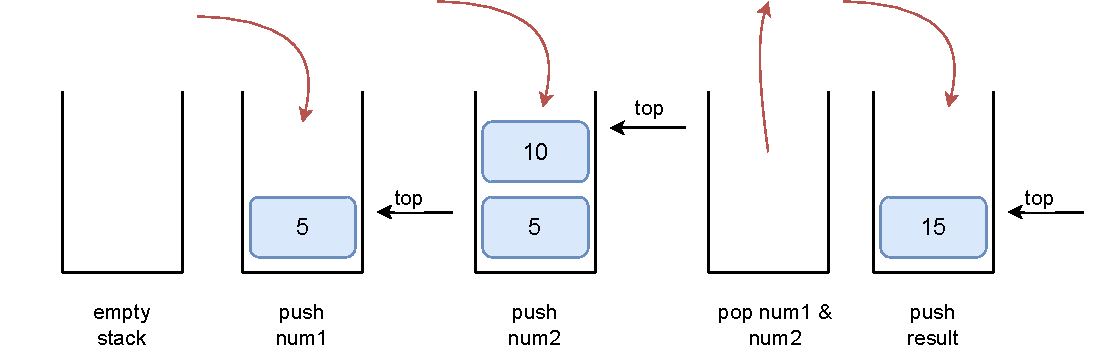
\includegraphics[width=1\linewidth]{images/wasm/stack_add_num_wasm.drawio.pdf}
  \caption{Visualization of how the stack is used to add two numbers in WebAssembly}
  \label{fig:stack_wasm_add_num}
\end{figure}